\documentclass[a4paper,margin=1cm,11pt]{report}
\usepackage[utf8]{inputenc}
\usepackage[T1]{fontenc}

%Pour modifier taille des sections et titres
%\usepackage{titlesec}

%\titleformat{\section}[block]{\Large\bfseries}{\thesection}{1em}{}

%package lien
\usepackage[colorlinks=true, linkcolor=blue]{hyperref}
\usepackage{graphicx}



% Title Page
\title{\Huge BOAT RACE}
\author{ALY Nandrasana \and Ange COLLETO}


\begin{document}
\maketitle

\tableofcontents
\newpage
\section*{Introduction}
\addcontentsline{toc}{section}{Introduction}
Ce projet de simulation de course de bateaux en C++ qu’on a nommé ‘BOAT RACE’ nous a permis de renforcer notre maîtrise dans l’utilisation du langage mais aussi d'élever nos compétences en programmation orientée objet. On a pu rencontrer de nouvelles bibliothèques qui sont SFML pour l’interface graphique et libphysics qui nous sert dans le réalisme physique pour la simulation. 
Ce rapport abordera d’abord les fonctionnalités mises en place dans l’application, ensuite nous illustrerons l’agencement du code et nous finirons avec la répartition des tâches.

\chapter{Les fonctionnalités de l'application}
\section{Simulation du comportement physique des bateaux}

Grâce à libphysics on a pu reproduire le comportement dynamique d’un bateau sous l’effet des forces (propulsion du moteur, le frottement avec l’eau, la rotation…).
Des méthodes sont intégrées dans la bibliothèque pour calculer les forces afin de les appliquer sur les caractéristiques physiques du bateau: vitesse linéaire, vitesse angulaire, position et orientation. 
Ainsi nous avons un comportement crédible de dérive, de rotation lente et d’inertie.
Bien que l’on dispose de méthodes pour nous permettre d’avoir des bateaux avec des caractéristiques personnalisées, on s’est limitée à la méthode de création de bateau générique contenu dans le fichier physicsEngine.h.

\section{Affichage graphique synchrone}
Nous avons représenté graphiquement le bateau avec un polygone simple, dont le barycentre est identifié au corps physique du bateau réel.
On a établi un facteur de conversion : 0.1.
En fonction des résultats des calculs des forces sur le corps physique du bateau, on convertit les positions et on dessine à nouveau chaque point du polygone selon les coordonnées du barycentre. Les transformations des points sont calculées via la rotation et la translation.
Ainsi on voit la position et l’orientation exactes des bateaux.

\section{Tableau de bord en temps réel}
Pour chaque bateau, on y a associé un tableau de bord qui nous permet d’afficher les données physiques en temps réel : vitesse, accélération, angle et rpm.

\section{Un menu interactif}
Point d’entrée du jeu, on veut différencier deux modes différents qui vont paramétrer l’environnement de course. L’application présente le mode “Single Player” et “Two Players”.
Le mode “Single Player” permet d’entrer dans une course avec seulement un bateau dessiné.
Le mode “Two Player” place deux joueurs côte à côte sur la ligne de départ.
Enfin le bouton ‘start’ permet de confirmer le choix et de lancer le jeu.

\section{Un environnement de course}
Après le choix du mode de jeu, on présente un environnement représentatif d’une course. Ainsi selon le mode choisi, on place le/les bateau(x) sur la ligne de départ. 
On a aussi établi des obstacles prédéfinis placés de façon pseudo-aléatoire sur la carte.
Il y a la présence également de signal de départ avec un feu multicolore. Enfin, on a placé la ligne d’arrivée.

\subsection{Commandes du jeu}
L’utilisateur peut diriger les bateaux.\\ 
Joueur 1:
\begin{itemize}
	\item Avancer: Z
	\item Reculer: S
	\item Rotation vers la droite : D
	\item Rotation vers la gauche : Q
\end{itemize}
Joueur 2:
\begin{itemize}
	\item Avancer: flèche haut
	\item Reculer: flèche bas
	\item Rotation vers la droite : flèche droite
	\item Rotation vers la gauche : flèche gauche
\end{itemize}

\subsection{Début de course}
Les commandes sont désactivées avant le signalement du départ. Un feu de 4 couleurs signale le départ imminent. Lorsque le feu est vert, on a un son qui est émis, les commandes sont activées et le chronomètre est lancé.

\subsection{Obstacles et Boosts}
Les obstacles empêchent les bateaux de traverser et ils sont directement stoppés. 
On a aussi créé des boosts style ‘Mario Kart’ pour permettre d’accélérer encore plus les bateaux.

\subsection{Fin de course}
\underline{Mode Single Player}\\
Quand le bateau franchit la ligne d’arrivée, un signal sonore est émis, les commandes sont désactivées et le résultat affiche le temps mis par le joueur pour traverser de la ligne de départ jusqu’à la ligne d’arrivée.\\\\
\underline{Mode Two Players}\\
Cas similaire quand l’un des deux bateaux franchit la ligne d’arrivée mais affiche en plus le gagnant, celui qui a franchi la ligne en premier.


\chapter{Choix de l'architecture}
Pour nous faciliter l’implémentation des fonctionnalités, on a opté pour une architecture orientée objet et modulaire. Cela permet de faire évoluer les fonctionnalités sans impacter les autres. Ainsi tout le projet est divisé en plusieurs classes et nous avons séparé les fichiers .hpp et .cpp. 

\begin{figure}[h]
	\centering
	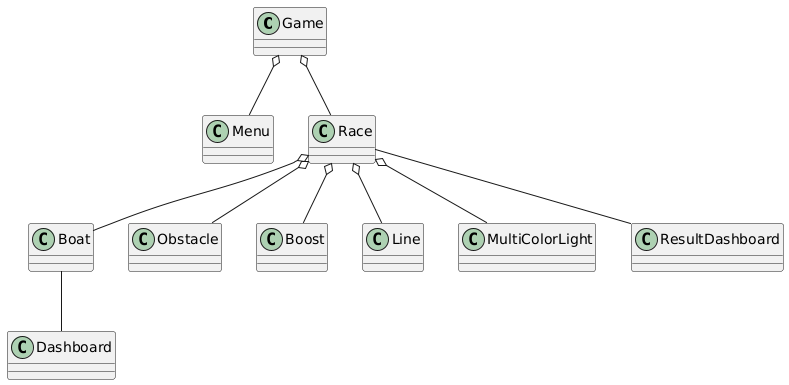
\includegraphics[width=0.5\textwidth]{diagrammeClasses}
	\caption{Diagramme de classes. *MultiColorLight=starting\_light}
	\label{fig:monimage}
\end{figure}


\section{Game}
Classe qui exécute la boucle du jeu et la gestion des fenêtres ou pages qui y sont associées (Menu et fenêtre de course).

\section{Menu}
Interface d’accueil et qui permet de choisir le mode de lancement de la course.

\section{Race}
Orchestre la course selon le mode choisi. Il a comme attributs principaux les bateaux et tout ce qui compose son environnement à savoir les obstacles et les lignes de départ et d’arrivée.
Elle met à jour tous les états de ces éléments et s’occupe du début et de la fin de la course. Elle gère aussi les intéractions entre les bateaux et les obstacles ou boosts.


\section{Boat}
Représente un bateau dans la simulation. Il y a donc son corps physique et les méthodes qui permettent d’y appliquer les forces et de mettre à jour ses caractéristiques.

\section{Obstacle}
Simple rectangle possédant une position, dimension et une couleur, à éviter.

\section{Boost}
Simple rectangle qui permet d’accélérer encore plus le bateau.

\section{Line}
Un rectangle allongé pour représenter la ligne de départ et la ligne d’arrivée.

\section{starting\_light}
Cercle qui change de couleur pour signaler le départ.

\section{Dashboard}
Interface qui affiche les données physiques en temps réel du bateau lors de son déplacement. Chaque bateau possède donc un seul dashboard.

\section{ResultDashboard}
Affiche les résultats à la fin de la course.

\chapter{Les difficultés rencontrées}

\section{Compilation et configuration avec CMake}
La configuration de CMake n’est pas très facile à appréhender dès le début. Heureusement que l’enseignant a fourni le support avec la configuration pour libphysics et sfml, puisque l’inclusion des bibliothèques est assez sensible. 
La compilation du code nous a pris presque tout le premier TP mais on arrive maintenant à s’y retrouver.

\section{Couplage entre la physique du bateau et son affichage graphique}
Associer le modèle physique du bateau à son sprite (image) SFML a demandé un travail d’adaptation. La classe Boat devait synchroniser la position et la rotation calculées par libphysics avec la représentation graphique. Cela a nécessité une conversion entre les coordonnées logiques et celles de la fenêtre SFML, ainsi qu'une gestion précise de l’angle pour faire pivoter le dessin.
Solution:
La première étape a été de choisir un facteur.
Puis comme on a voulu coupler le barycentre du polygone avec le corps, physique, on a gardé les coordonnées relatives des points du polygone par rapport au barycentre.
A chaque frame on recalcule donc les positions des points en y appliquant les mêmes transformations que celles du barycentre.

\section{Calcul des forces et compréhension du modèle dynamique}
Comprendre et utiliser les données physiques du bateau (accélérations, vitesse, couple) n'était pas trivial. Nous avons sollicité le prof pour nous préciser l’utilisation des modèles de libphysics et un peu de documentation a été nécessaire.

\section{Gestion de la bibliothèque dynamique}
Une erreur a persisté lors du lancement de l'exécutable : la non détection de bibliothèque physique liblibphysicsd.so. Le système n’a pas trouvé la bibliothèque partagée.

\chapter{Travail de groupe}
On a réparti efficacement les tâches tout en gardant une collaboration étroite à chaque étape de développement. Voici comment nous avons organisé le travail:\\
ALY s’est principalement concentré sur :
\begin{itemize}
	\item La conception des classes
	\item L’interface utilisateur (menus, dashboard, feu tricolore, résultats)
	\item La gestion des états du jeu et des transitions (départ, arrivée, scores)
	\item L’intégration de l’audio et des polices\\
\end{itemize}
COLLETTO s’est chargé de :
\begin{itemize}
	\item La gestion des événements clavier
	\item Le couplage entre la physique et la représentation graphique
	\item Les intéractions entre les objets de liés à la course (bateau, lignes départ/arrivée, obstacles, boosts)
	\item Gestion des calculs des forces
\end{itemize}

\newpage
\section*{Conclusion}
\addcontentsline{toc}{section}{Conclusion}
Ce projet de simulation a été riche en apprentissage, notamment sur le plan technique. Il nous a permis d’explorer les différentes facettes du développement logiciel en C++, depuis la conception orientée objet jusqu’à l’intégration de bibliothèques externes comme SFML et libphysics. 
Nous avons su mettre en œuvre une architecture modulaire et évolutive en nous appuyant sur des concepts solides de programmation : séparation des responsabilités, logique événementielle, gestion des ressources et rendu temps réel. L’utilisation de CMake pour la compilation multi-fichiers ainsi que l’emploi de bibliothèques dynamiques nous ont confrontés à des défis techniques, que nous avons su surmonter progressivement.
Enfin, ce projet constitue une base solide que nous pourrions enrichir à l’avenir avec des fonctionnalités supplémentaires telles qu’un mode multijoueur en ligne, des cartes aléatoires ou un éditeur de circuits.


\end{document}          
